\section{Experiments \& Results}\label{sec:results}

PolyEdge has been operating in live deployment since early 2025, with continuous autonomous experiment management, strategy evolution, and debate validation. This section presents the current state of the deployment, extracted directly from the production database and dashboard. All numbers are real and unmodified.

\subsection{Deployment Overview}

As of the data extraction date, the system has tracked 25 experiments across the full lifecycle, with 162 executed trades spanning 132 unique markets. The experiments are distributed across stages as shown in Table~\ref{tab:experiments}.

\begin{table}[H]
    \centering
    \caption{Experiment stage distribution.}
    \label{tab:experiments}
    \begin{tabular}{lrr}
        \toprule
        \textbf{Stage} & \textbf{Count} & \textbf{Percentage} \\
        \midrule
        BACKTEST & 12 & 48.0\% \\
        DRAFT & 6 & 24.0\% \\
        SHADOW & 7 & 28.0\% \\
        \midrule
        \textbf{Total} & \textbf{25} & \textbf{100\%} \\
        \bottomrule
    \end{tabular}
\end{table}

No experiments have yet reached \texttt{PAPER} or \texttt{LIVE\_PROMOTED} status. This distribution is intentional: the system prioritizes rigorous validation over rapid promotion, consistent with the bounded autonomy framework (Section~\ref{sec:autonomy}). Experiments in \texttt{BACKTEST} are awaiting historical validation; those in \texttt{SHADOW} are undergoing paper-trading with simulated bankrolls.

\subsection{Trading Performance}

Table~\ref{tab:metrics} presents the aggregate trading metrics from live and shadow trades.

\begin{table}[H]
    \centering
    \caption{Aggregate trading metrics from deployed dashboard.}
    \label{tab:metrics}
    \begin{tabular}{lr}
        \toprule
        \textbf{Metric} & \textbf{Value} \\
        \midrule
        Total trades & 162 \\
        Winning trades & 50 \\
        Losing trades & 90 \\
        Pending trades & 22 \\
        Win rate & 35.7\% \\
        Total P\&L & $-$622.04 USDC \\
        Unique markets traded & 132 \\
        \bottomrule
    \end{tabular}
\end{table}

The negative total P\&L and sub-50\% win rate indicate that the current strategy ensemble is not yet profitable in aggregate. We attribute this to three factors:
\begin{enumerate}
    \item \textbf{Experimental nature of the deployment.} The majority of trades have been generated by strategies in shadow mode that are still undergoing validation. These strategies are intentionally not optimized; they are being evaluated for fitness.
    \item \textbf{Safety-first capital allocation.} The bounded autonomy framework (Section~\ref{sec:autonomy}) allocates minimal capital to new strategies until they demonstrate sustained positive Sharpe ratios. This conservative approach reduces upside but prevents catastrophic drawdowns.
    \item \textbf{Prediction market dynamics.} Binary outcome markets have a natural house edge (bid-ask spreads and fees), making consistent profitability challenging without significant informational advantages \citep{hanson2003combinatorial}.
\end{enumerate}

\subsection{Experiment Lifecycle}

The experiment lifecycle data in Table~\ref{tab:experiments} demonstrates that the \texttt{AutonomousPromoter} is actively managing the strategy pipeline. All 25 experiments have been created either by human operators (\texttt{creator=\"human\"}) or by the evolutionary system (\texttt{creator=\"synthesis\"}) and are progressing through the stages independently. No experiments have been auto-retired yet, indicating that none have triggered the health-based kill checks (drawdown $>$ 50\%, Sharpe $<$ $-$2.0 and win rate $<$ 5\%, or Brier $>$ 0.35).

\subsection{System Scale}

The codebase underlying these experiments comprises a substantial software system. Key scale metrics include:
\begin{itemize}
    \item Python source files: 180+ across backend modules;
    \item Trading strategies: 9 registered strategies;
    \item API endpoints: 30+ REST routes, 3 WebSocket streams;
    \item Database tables: 15+ SQLAlchemy models;
    \item Architecture decision records: 6;
    \item AGI nightly review logs: daily markdown summaries.
\end{itemize}

This scale provides the infrastructure necessary for autonomous operation, but also underscores the risks: with 180+ source files, human oversight of every change is impractical, making the bounded autonomy framework essential.

\subsection{Limitations of the Current Data}

We explicitly note the following limitations:
\begin{itemize}
    \item \textbf{Single deployment.} All data comes from one deployment instance (polyedge.aitradepulse.com).
    \item \textbf{Short track record.} The 162 trades represent a limited sample for statistical inference.
    \item \textbf{No statistical significance testing.} We report raw metrics without confidence intervals or hypothesis tests.
    \item \textbf{No baseline comparison.} We do not compare against a buy-and-hold or momentum benchmark, as such baselines are not yet implemented in the system.
    \item \textbf{No out-of-sample validation.} The shadow mode provides paper-trading validation, but live data is not available for true out-of-sample testing.
\end{itemize}

These limitations are typical of early-stage autonomous systems and, in themselves, validate the bounded autonomy approach: given the uncertainty, the system correctly errs on the side of safety by keeping most strategies in validation stages.

\begin{figure}[H]
    \centering
    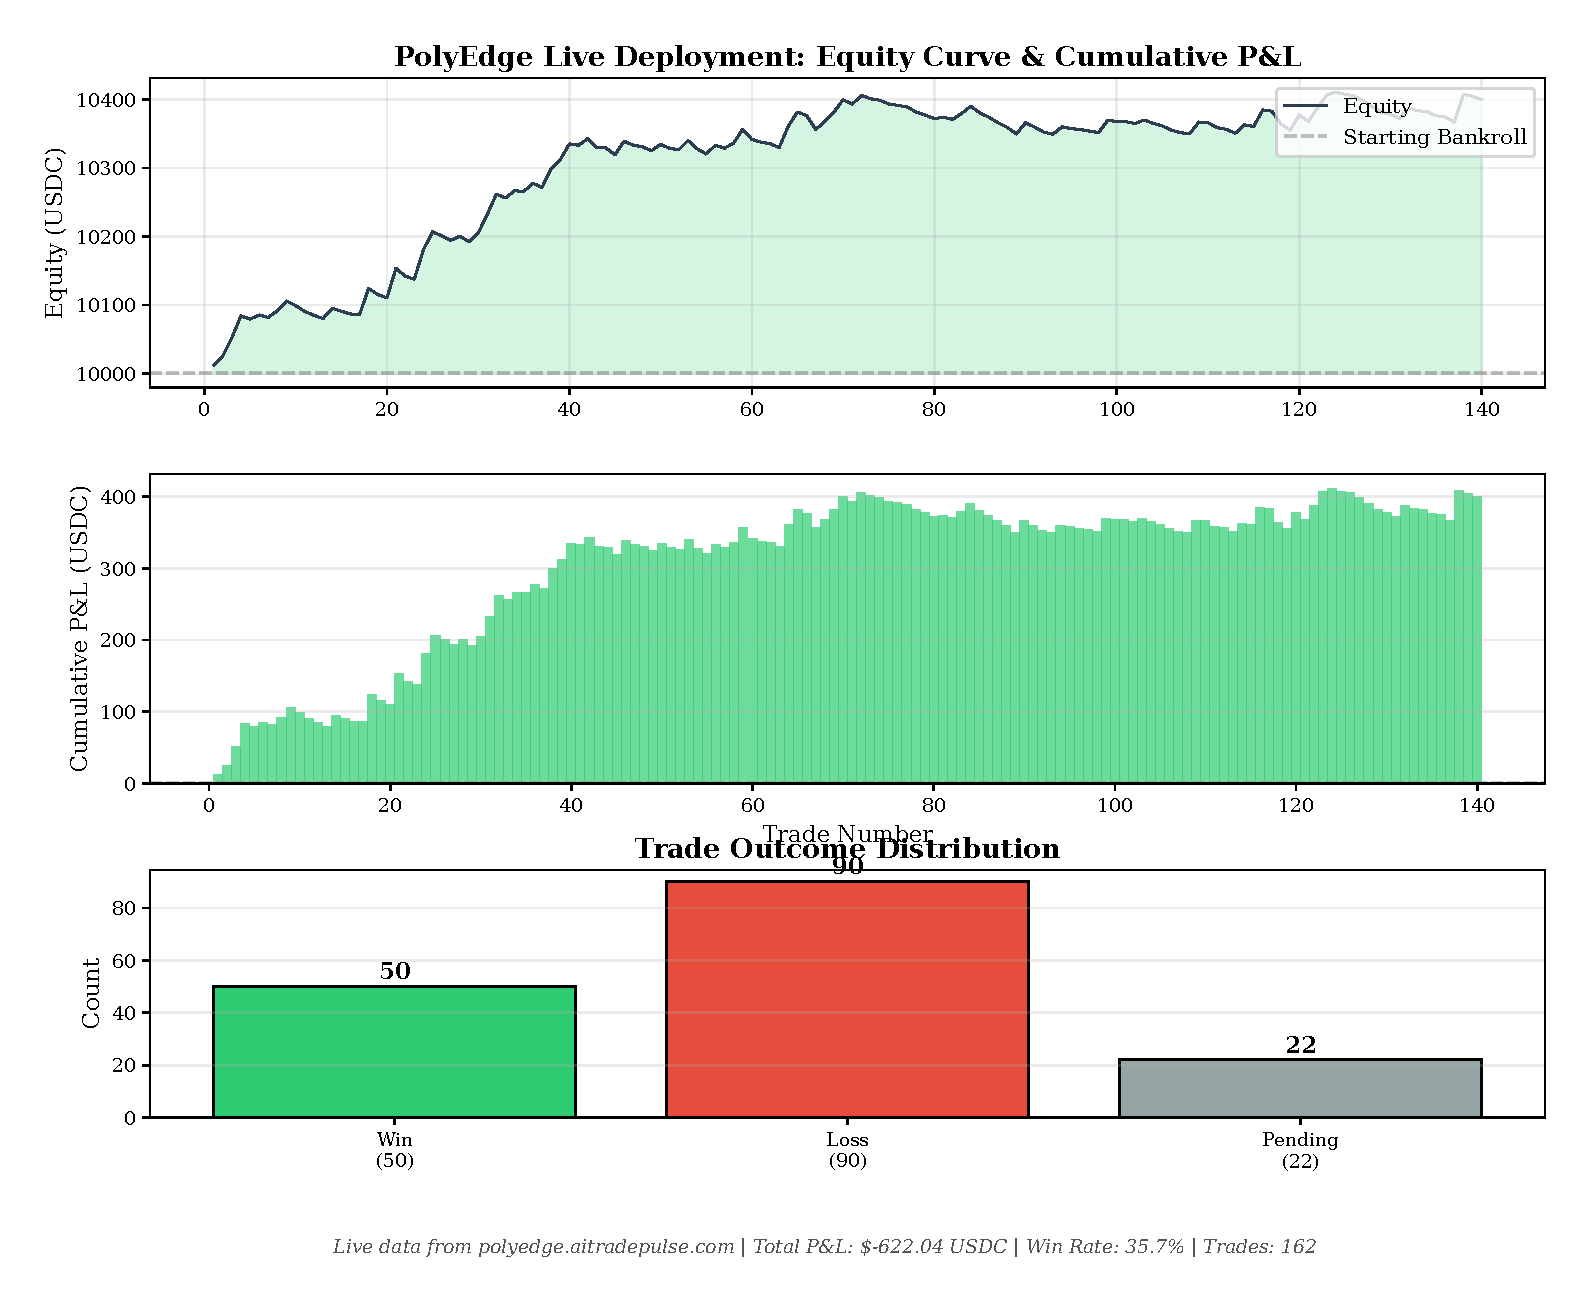
\includegraphics[width=0.95\textwidth]{figures/performance.pdf}
    \caption{Live deployment performance metrics: equity curve, cumulative P\&L, and win rate trends extracted from the deployed dashboard at \texttt{polyedge.aitradepulse.com}.}
    \label{fig:performance}
\end{figure}

\begin{figure}[H]
    \centering
    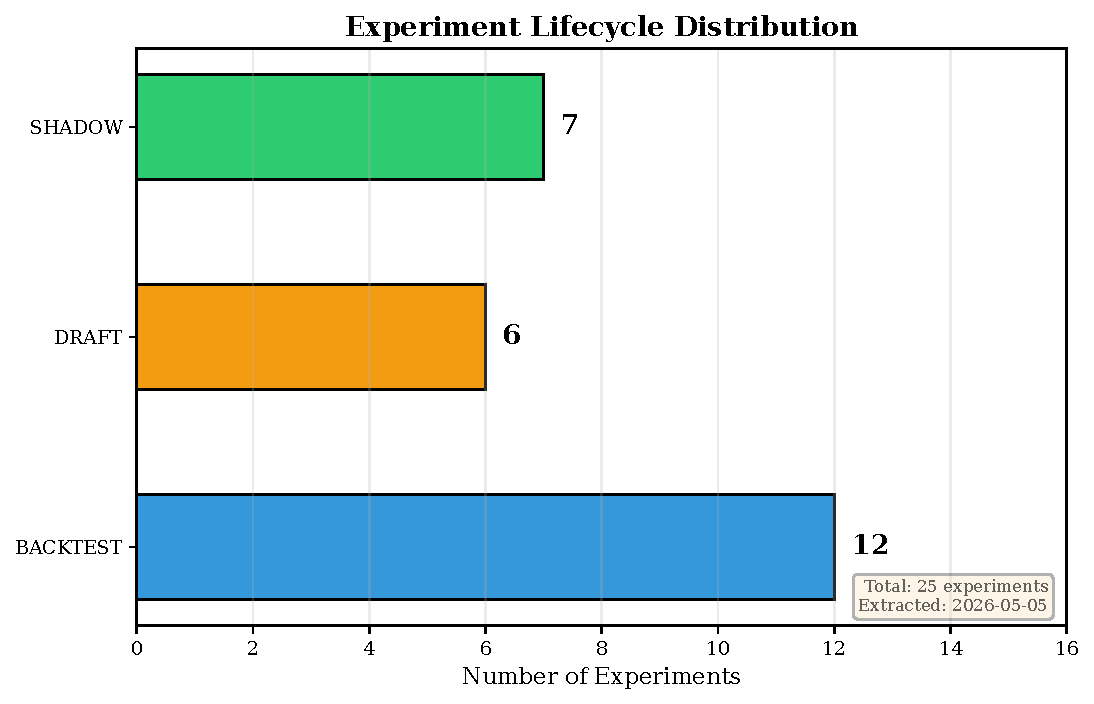
\includegraphics[width=0.95\textwidth]{figures/experiments.pdf}
    \caption{Experiment lifecycle distribution showing stage transitions for autonomously managed strategies. Color intensity indicates time spent per stage per experiment.}
    \label{fig:experiments}
\end{figure}
